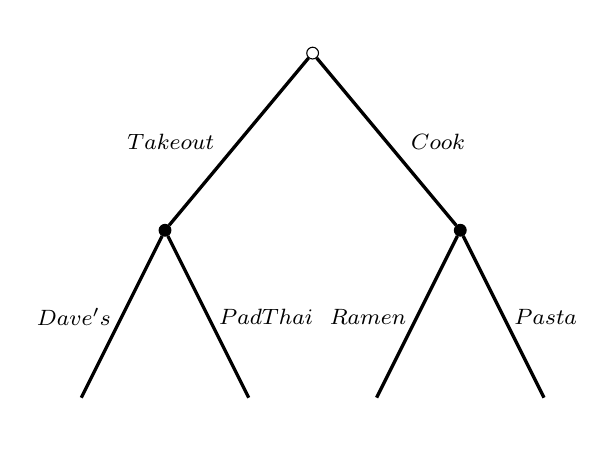
\begin{tikzpicture}[scale=1.5,font=\footnotesize, edge from parent/.style={draw, very thick}]
    \tikzstyle{solid node}=[circle,draw,inner sep=1.5,fill=black]
    \tikzstyle{hollow node}=[circle,draw,inner sep=1.5]
    \tikzstyle{level 1}=[level distance=15mm,sibling distance=2.5cm]
    \tikzstyle{level 2}=[level distance=15mm,sibling distance=1.5cm]
    \tikzstyle{level 3}=[level distance=15mm,sibling distance=1cm]
    
    \node(0)[hollow node,label=above:{}]{}
        child{node(1)[solid node,label=above left:{}]{}
            child{node[label=below:{}]{} edge from parent node[left]{$Dave's$}}
            child{node[label=below:{}]{} edge from parent node[right]{$Pad Thai$}}
            edge from parent node[left,xshift=-5]{$Takeout$}
        }
        child{node(2)[solid node,label=above right:{}]{}
            child{node[label=below:{}]{} edge from parent node[left]{$Ramen$}}
            child{node[label=below:{}]{} edge from parent node[right]{$Pasta$}}
            edge from parent node[right,xshift=5]{$Cook$}
        };

    %\draw[<-,>=latex, color=blue](0)--(8:8mm)node[inner sep=0,right]{Initial Node};
    %\draw[<-, >=latex, color=blue](1)--(-20:20mm)node[inner sep=0, right]{Decision Nodes};
    %\draw[<-,>=latex, color=blue](2)--(-20:20mm){};
    %\draw[<-,>=latex, color=blue](0)--(-20:20mm){};
\end{tikzpicture}
